\documentclass[journal,12pt,twocolumn]{IEEEtran}
\usepackage{setspace}
\usepackage{gensymb}
\usepackage{xcolor}
\usepackage{caption}
\singlespacing
\usepackage{siunitx}
\usepackage[cmex10]{amsmath}
\usepackage{mathtools}
\usepackage{hyperref}
\usepackage{amsthm}
\usepackage{mathrsfs}
\usepackage{txfonts}
\usepackage{stfloats}
\usepackage{cite}
\usepackage{cases}
\usepackage{subfig}
\usepackage{longtable}
\usepackage{multirow}
\usepackage{enumitem}
\usepackage{bm}
\usepackage{mathtools}
\usepackage{listings}
\usepackage{tikz}
\usetikzlibrary{shapes,arrows,positioning}
\usepackage{circuitikz}
\renewcommand{\vec}[1]{\boldsymbol{\mathbf{#1}}}
\DeclareMathOperator*{\Res}{Res}
\renewcommand\thesection{\arabic{section}}
\renewcommand\thesubsection{\thesection.\arabic{subsection}}
\renewcommand\thesubsubsection{\thesubsection.\arabic{subsubsection}}

\renewcommand\thesectiondis{\arabic{section}}
\renewcommand\thesubsectiondis{\thesectiondis.\arabic{subsection}}
\renewcommand\thesubsubsectiondis{\thesubsectiondis.\arabic{subsubsection}}
\hyphenation{op-tical net-works semi-conduc-tor}

\lstset{
language=Python,
frame=single, 
breaklines=true,
columns=fullflexible
}
\begin{document}
\theoremstyle{definition}
\newtheorem{theorem}{Theorem}[section]
\newtheorem{problem}{Problem}
\newtheorem{proposition}{Proposition}[section]
\newtheorem{lemma}{Lemma}[section]
\newtheorem{corollary}[theorem]{Corollary}
\newtheorem{example}{Example}[section]
\newtheorem{definition}{Definition}[section]
\newcommand{\BEQA}{\begin{eqnarray}}
\newcommand{\EEQA}{\end{eqnarray}}
\newcommand{\define}{\stackrel{\triangle}{=}}
\newcommand{\myvec}[1]{\ensuremath{\begin{pmatrix}#1\end{pmatrix}}}
\newcommand{\mydet}[1]{\ensuremath{\begin{vmatrix}#1\end{vmatrix}}}
\bibliographystyle{IEEEtran}
\providecommand{\nCr}[2]{\,^{#1}C_{#2}} % nCr
\providecommand{\nPr}[2]{\,^{#1}P_{#2}} % nPr
\providecommand{\mbf}{\mathbf}
\providecommand{\pr}[1]{\ensuremath{\Pr\left(#1\right)}}
\providecommand{\qfunc}[1]{\ensuremath{Q\left(#1\right)}}
\providecommand{\sbrak}[1]{\ensuremath{{}\left[#1\right]}}
\providecommand{\lsbrak}[1]{\ensuremath{{}\left[#1\right.}}
\providecommand{\rsbrak}[1]{\ensuremath{{}\left.#1\right]}}
\providecommand{\brak}[1]{\ensuremath{\left(#1\right)}}
\providecommand{\lbrak}[1]{\ensuremath{\left(#1\right.}}
\providecommand{\rbrak}[1]{\ensuremath{\left.#1\right)}}
\providecommand{\cbrak}[1]{\ensuremath{\left\{#1\right\}}}
\providecommand{\lcbrak}[1]{\ensuremath{\left\{#1\right.}}
\providecommand{\rcbrak}[1]{\ensuremath{\left.#1\right\}}}
\theoremstyle{remark}
\newtheorem{rem}{Remark}
\newcommand{\sgn}{\mathop{\mathrm{sgn}}}
\newcommand{\rect}{\mathop{\mathrm{rect}}}
\newcommand{\sinc}{\mathop{\mathrm{sinc}}}
\providecommand{\abs}[1]{\left\vert#1\right\vert}
\providecommand{\res}[1]{\Res\displaylimits_{#1}} 
\providecommand{\norm}[1]{\lVert#1\rVert}
\providecommand{\mtx}[1]{\mathbf{#1}}
\providecommand{\mean}[1]{E\left[ #1 \right]}
\providecommand{\fourier}{\overset{\mathcal{F}}{ \rightleftharpoons}}
\providecommand{\ztrans}{\overset{\mathcal{Z}}{ \rightleftharpoons}}
\providecommand{\system}[1]{\overset{\mathcal{#1}}{ \longleftrightarrow}}
\newcommand{\solution}{\noindent \textbf{Solution: }}
\providecommand{\dec}[2]{\ensuremath{\overset{#1}{\underset{#2}{\gtrless}}}}
\let\StandardTheFigure\thefigure
\def\putbox#1#2#3{\makebox[0in][l]{\makebox[#1][l]{}\raisebox{\baselineskip}[0in][0in]{\raisebox{#2}[0in][0in]{#3}}}}
     \def\rightbox#1{\makebox[0in][r]{#1}}
     \def\centbox#1{\makebox[0in]{#1}}
     \def\topbox#1{\raisebox{-\baselineskip}[0in][0in]{#1}}
     \def\midbox#1{\raisebox{-0.5\baselineskip}[0in][0in]{#1}}

\vspace{3cm}
\title{Conic Assignment}
\author{Gautam Singh}
\maketitle
\bigskip

\begin{abstract}
    This document contains the solution to Question 12 of Exercise 2 in Chapter
    11 of the class 11 NCERT textbook.
\end{abstract}

\begin{enumerate}
    \item Find the equation of the parabola with vertex
    \begin{align}
        \vec{P} = \myvec{0\\0}
    \end{align}
    and passing through the point
    \begin{align}
        \vec{Q} = \myvec{5\\2}
    \end{align}
    and symmetric to the $y$-axis.

    \solution Let the equation of the conic with focus $\vec{F}$, directrix
    $\vec{n}^\top\vec{x} = c$ and eccentricity $e$ be
    \begin{align}
        \vec{x}^\top\vec{V}\vec{x} + 2\vec{u}^\top\vec{x} + f = 0
        \label{eq:conic-def}
    \end{align}
    where
    \begin{align}
        \vec{V} &\triangleq \norm{\vec{n}}^2\vec{I} - e^2\vec{n}\vec{n}^\top \label{eq:V-def} \\
        \vec{u} &\triangleq ce^2\vec{n} - \norm{\vec{n}}^2\vec{F} \label{eq:u-def} \\
        f &\triangleq \norm{\vec{n}}^2\norm{\vec{F}}^2 - c^2e^2 \label{eq:f-def}
    \end{align}
    Since the conic is a parabola symmetric to the $y$-axis, we have
    \begin{align}
        \vec{n} = \myvec{0\\1},\ e = 1
    \end{align}
    and also that $\vec{F}$ lies on the $y$-axis. From \eqref{eq:V-def},
    \begin{align}
        \vec{V} &= \vec{I} - \myvec{0&0\\0&1} = \myvec{1&0\\0&0} \label{eq:V-val} \\
        \vec{u} &= c\myvec{0\\1} - \vec{F} \label{eq:u-val} \\
        f &= \norm{\vec{F}}^2 - c^2
    \end{align}
    Putting $\vec{x} = \vec{P}$ in \eqref{eq:conic-def} gives $f = 0$, thus 
    \begin{align}
        \norm{\vec{F}}^2 = c^2
        \label{eq:F-c}
    \end{align}
    Putting $\vec{x} = \vec{Q}$ in \eqref{eq:conic-def}, using \eqref{eq:V-val}, 
    \eqref{eq:u-val} and noting that $f = 0$, we get
    \begin{align}
        &\myvec{5&2}\myvec{1&0\\0&0}\myvec{5\\2} + 2\brak{c\myvec{0&1}-\vec{F}^\top}\myvec{5\\2} = 0 \\
        &\implies 25 + 4c - 2\vec{F}^\top\myvec{5\\2} = 0 \\
        &\implies \vec{F}^\top\myvec{5\\2} = \frac{25}{2} + 2c \label{eq:p1} \\
        &\implies \vec{F} = \myvec{0\\\frac{25}{4}+c} \label{eq:F-coords}
    \end{align}
    since $\vec{F}$ lies on the $y$-axis as remarked before. Using 
    \eqref{eq:F-c},
    \begin{align}
        \frac{25}{4}+c\pm c &= 0 \\
        \implies c &= -\frac{25}{8}
    \end{align}
    Thus,
    \begin{align}
        \vec{F} = \myvec{0\\\frac{25}{8}}
    \end{align}
    Substituting into \eqref{eq:u-def},
    \begin{align}
        \vec{u} = -\frac{25}{8}\myvec{0\\1} - \myvec{0\\\frac{25}{8}} = \myvec{0\\-\frac{25}{4}}
    \end{align}
    And the equation of the conic is given by
    \begin{align}
        \vec{x}^\top\myvec{1&0\\0&0}\vec{x} - \frac{25}{2}\myvec{0&1}\vec{x} = 0
    \end{align}
    The conic is plotted in Fig. \ref{fig:conic} using the Python code 
    \texttt{codes/conic.py}.
    \begin{figure}[!ht]
        \centering
        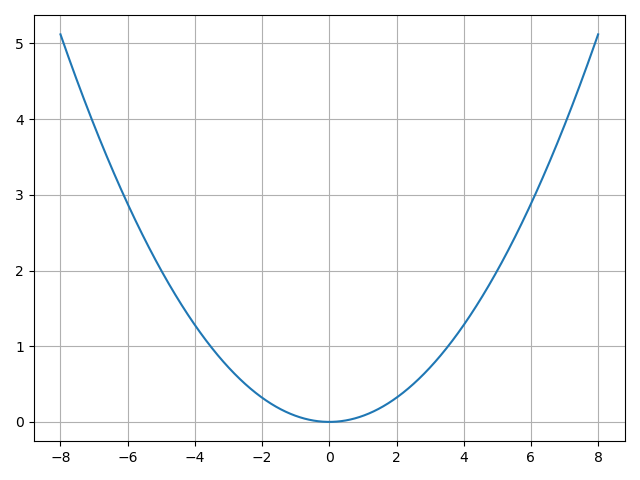
\includegraphics[width=\columnwidth]{figs/conic.png}
        \caption{Locus of the required parabola.}
        \label{fig:conic}
    \end{figure}
\end{enumerate}
\end{document}
